\labwork{Установка ПО ST-Link для \vld}\label{labinststsoft}

\menu{\wcmd{\url{http://www.google.com}}>ST-Link>ST-Link - STMicroelectronics}

\bigskip
\begin{tabular}{l l l}
\menu{STSW-LINK002>Download}	&ST-LINK USB driver for Windows XP&драйвер\\
\menu{STSW-LINK004>Download}	&STM32 ST-LINK utility&ПО программатора\\
\end{tabular}

\bigskip
\menu{\file{st-link\_usbdriver.zip}>\file{ST-Link\_USBdriver.exe}}

\menu{STLinkDriver>Welcome>Next>Install
to>\file{C:/ARM/STM32/STdriver}>Next>Install>Finish}

\bigskip
\menu{\file{stsw-link004.zip}>\file{STM32 ST-LINK Utility\_v3.4.0.exe}}

\menu{ST-LINK
Utility>Next>License>Yes>Distination>\file{C:/ARM/STM32/STLinkUtil}>Finish}

\menu{(сам запустился) Device Driver Install Wizard>Далее>Установить}

\bigskip
\menu{\winstart>STMicroelectronics>ST-LINK Utility>STM32 ST-Link}

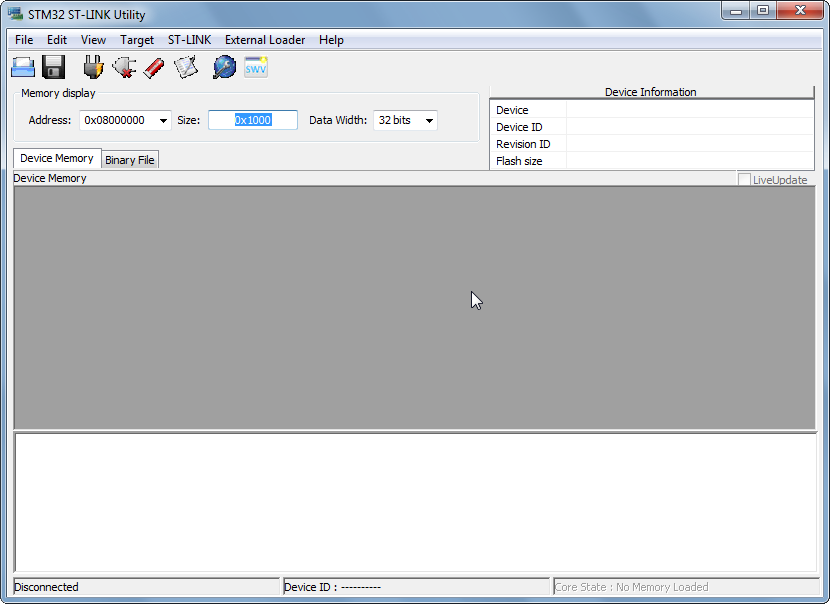
\includegraphics[height=0.5\textheight]{fig/stlink0.png}

\bigskip
\menu{STutil>Target>Connect}

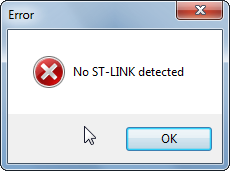
\includegraphics[height=0.2\textheight]{fig/nostlink.png}

\bigskip
Подключаем плату \vld\ кабелем, в системе подключается новое устройство,
на плате запускается ранее залитая в МК прошивка:

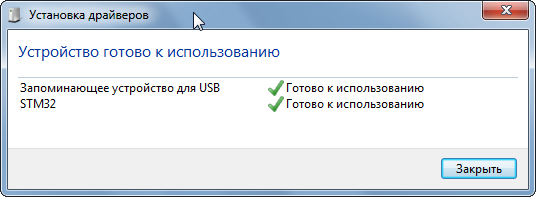
\includegraphics[height=0.3\textheight]{fig/stdrvok.png}

\bigskip
\menu{STutil>Target>Connect}

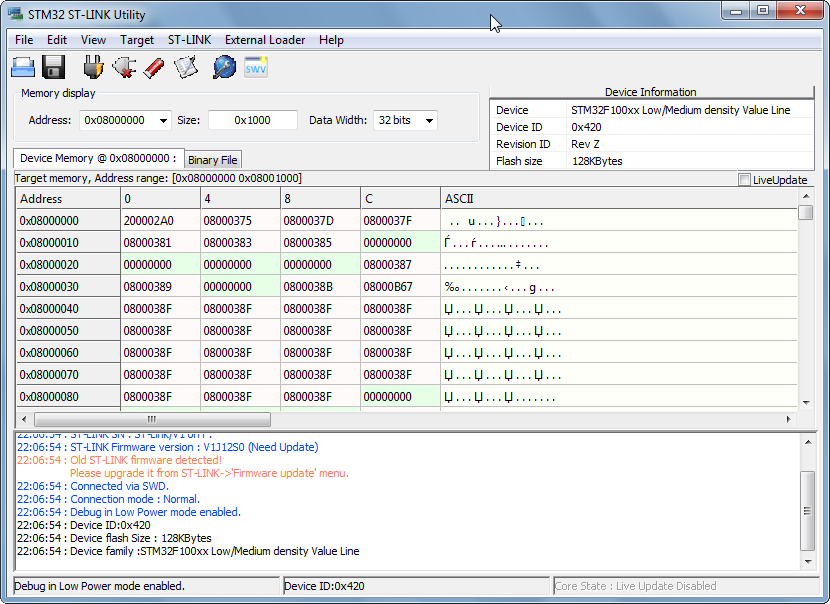
\includegraphics[width=0.9\textwidth]{fig/stconnected.png}

\bigskip
Обновление прошивки ST-Link:

\menu{ST Link>ST-LINK>Firmware update>Device Connect>not in DFU
mode}

\menu{передергиваем плату>Device connect>Upgrade to V.1.J13.S0>Yes}

\bigskip


